
\documentclass[12pt,article]{memoir}

\usepackage{fancyhdr}
\usepackage{graphicx}
\usepackage{fontspec}
\setmainfont{Calibri}
\usepackage{tikz}
\usetikzlibrary{calc}
\usepackage{xcolor}
\usepackage{xpatch}
\usepackage{hyperref}

\usepackage{fancyhdr}
\usepackage{graphicx}
\usepackage{fontspec}
\setmainfont{Calibri}
\usepackage{tikz}
\usetikzlibrary{calc}
\usepackage{xcolor}
\usepackage{xpatch}
\usepackage{hyperref}
\usepackage{tabu}
\usepackage{float}
\usepackage[autostyle, english = american]{csquotes}
\usepackage{gensymb}


\usepackage[yyyymmdd]{datetime} % change date format to yyyy/mm/dd to fit ISO8601

\renewcommand{\familydefault}{\sfdefault} % set font
\renewcommand{\dateseparator}{--} % change date-seperators to - to fit ISO8601

\renewcommand\contentsname{Table of Contents}

\chapterstyle{section}
\renewcommand*{\chapnumfont}{\normalfont\HUGE\bfseries\sffamily}
\renewcommand*{\chaptitlefont}{\normalfont\HUGE\bfseries\sffamily}

\makeatletter 
% define macro for itemcode
\newcommand\itemcode[1]{\renewcommand\@itemcode{#1}}
\newcommand\@itemcode{}

% define macro for rev number
\newcommand\revnumber[1]{\renewcommand\@revnumber{#1}}
\newcommand\@revnumber{}
\makeatother

\definecolor{orbitOrange}{RGB}{250,62,0} % the ORBiT orange

\setlrmarginsandblock{2.5cm}{2.5cm}{*}
\setulmarginsandblock{2.5cm}{*}{1}
\checkandfixthelayout 

\setlength{\beforechapskip}{0cm} % reduce chapter spacing

\hypersetup{
    colorlinks,
    citecolor=black,
    filecolor=black,
    linkcolor=black,
    urlcolor=black
}

%**********************************************************************
%Document titles etc. defined here: (replace [] as well)
\title{ORBiT Avionics System II Requirements}
\author{Jinzhi Cai}
\itemcode{ER00002}
\revnumber{A03}
\date{\today}
%end of document titles etc.
%**********************************************************************

\makeatletter
\let\runtitle\@title
\let\runitemcode\@itemcode
\makeatother

% set header style
\pagestyle{fancy}
{
	\fancyheadoffset{0cm}

	\lhead{\runtitle \ - \runitemcode}
	\rhead{Page: \thepage }
	%\chead{\leftmark} % section name
}

\newcommand{\OrbitBackground}{% For a logo drawn with TikZ
\begin{tikzpicture}[remember picture,overlay] % draw background
	\coordinate (bl) at (current page.south west);
	\coordinate (r) at (current page.east);
    \coordinate (A) at ($(bl)+(0,3cm)$);
    \coordinate (B) at ($(r)+(0,-2cm)$);
    \coordinate (C) at (current page.south east);
    \coordinate (ctrlNode) at ($(current page.south) + (0cm,1cm)$);
    \coordinate (ctrlNode2) at ($(current page.south east) + (-1cm,1cm)$);
    \fill[orbitOrange, fill opacity=0.2]
    (A) .. controls (ctrlNode) and (ctrlNode2) .. (B) -- (C) -- (bl);
    \node [white] at ($(C) + (-3cm,1cm)$) {2015-\the\year \ ORBiT@SU};
\end{tikzpicture}
}

\cfoot{\OrbitBackground}

\begin{document}

\begin{tikzpicture}[remember picture,overlay] % draw background
	\coordinate (bl) at (current page.south west);
	\coordinate (r) at (current page.east);
    \coordinate (A) at ($(bl)+(0,3cm)$);
    \coordinate (B) at ($(r)+(0,-2cm)$);
    \coordinate (C) at (current page.south east);
    \coordinate (ctrlNode) at ($(current page.south) + (0cm,1cm)$);
    \coordinate (ctrlNode2) at ($(current page.south east) + (-1cm,1cm)$);
    \fill[orbitOrange]
    (A) .. controls (ctrlNode) and (ctrlNode2) .. (B) -- (C) -- (bl);
    \node [white] at ($(C) + (-3cm,1cm)$) {2015-\the\year \ ORBiT@SU};
\end{tikzpicture}

\makeatletter

\includegraphics[width=\textwidth]{../logo.jpg}\\[4ex]
\begin{center}
	\bfseries \fontsize{50}{50}\selectfont  \@title \\[2ex]
	\LARGE  \@itemcode
\end{center}
\vfill
\begin{flushright}
	\LARGE Rev: \@revnumber\\
	\large \@author\\
	\large \@date\\[18ex]
\end{flushright}
\makeatother
\thispagestyle{empty}
\newpage

\tableofcontents*
\thispagestyle{fancy}
\newpage

%**********************************************************************
% Everything after this is the main document. Edit below this line,

\chapter{Introduction}
\section{Scope}
This document covers high level requirements of the ORBiT Avionics System II. This includes the system components, overall functionality, and mechanical constraints.

\section{Purpose}
The ORBiT Avionics System II (OA-II) is the next generation avionics system for the Orange Rocket Ballistics Team experimental hybrid rocket. It include two major assemblies, the Vehicle Electronics, and the Base Station Electronics. It also includes a Ground Test System and a Radio Communications system.\\
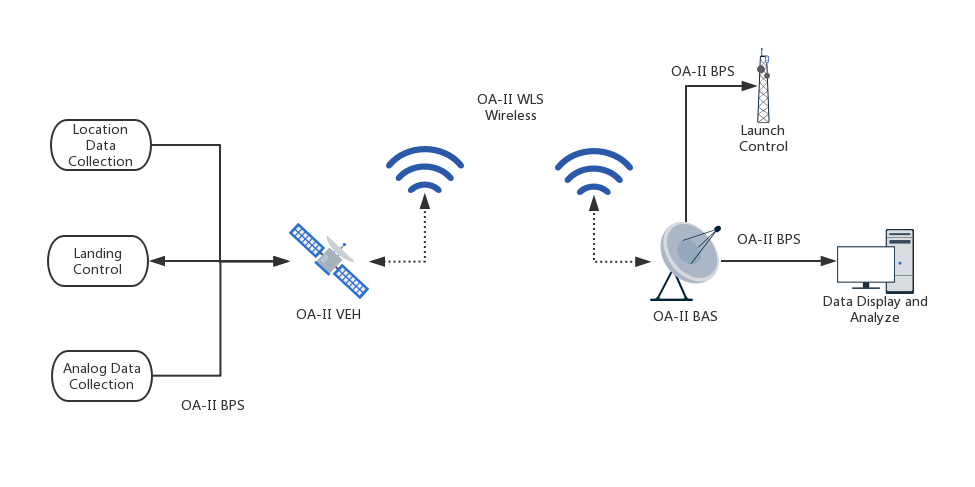
\includegraphics[width=\textwidth]{sys_diag.png}

\section{Revision History}
\begin{table}[H]
	\centering
	\begin{tabu}{r || c | c | c | c }
		Rev & Author & Approver & Changes & Date\\ \hline
		A01 & Jinzhi Cai & & Initialize  & 2019-06-21 \\
		-	& Jinzhi Cai & & Add Radio requirement & 2019-06-24 \\ \hline
		A02 & Gabriel Smolnycki & & Edits for clarity & 2019-06-25\\ \hline
		A03 & Jinzhi Cai & & Add Engine Testing System & 2019-07-04\\ \hline
		A04 & Gabriel Smolnycki & & \shortstack{Formatting and consistency\\with system architecture} & 2019-07-08\\
	\end{tabu}
	\caption{Summary of Revision History}
	\label{tab:rev}
\end{table}

\newpage

\chapter{System Description}
\subsection{Vehicle Electronics (VEH)}
The OA-II VEH is used to control the rocket's various subsystems, collect information about the rocket's performance, and communicate this with the BAS for remote control and monitoring. It also has autonomous software and onboard storage, to allow for continued operation in case of wireless link failure.
\begin{itemize}
	\item Data receiving and transmission to base station
	\item 3D linear kinematics data.
	\begin{itemize}
		\item $X$, $Y$, $Z$ (position)
		\item $V_X$, $V_Y$, $V_Z$ (velocity)
		\item $A_X$, $A_Y$, $A_Z$ (acceleration)
	\end{itemize}
	\item 3D rotational kinematics data
	\begin{itemize}
		\item $\theta_X$, $\theta_Y$, $\theta_Z$ (position)
		\item $\omega_X$, $\omega_Y$, $\omega_Z$ (velocity)
		\item $\alpha_X$, $\alpha_Y$, $\alpha_Z$ (acceleration)
	\end{itemize}
	\item Static and dynamic air pressure
	\item Redundant 28V power supplies and power management
	\item Failsafe capability
	\item High frequency data collection ($F_s \geq 10kHz$, $ENOB \geq 8$)
	\item Actuator and ignitor control ($P_{pk} \geq 50W$)
	\item 1080p 60Hz RGB Camera $\times$ 4
	\item Low power Doppler radio location beacon
	\begin{itemize}
		\item 24hr battery life
		\item 5km range
	\end{itemize}
	\item Built-in self test (BIST)
	\item Conformal coating
	\item Operation over extended 0-85\degree C temperature range
\end{itemize}

\subsection{Base Station Electronics (BAS)}
The OA-II BAS is used to communicate with the VEH and perform basic realtime analysis on rocket telemetry data. The BAS provides live location and performance information, and data storage for further analysis. The BAS can also help to locate the rocket after landing.
\begin{itemize}
	\item Data receiving and transmission to vehicle
	\item Display vehicle status information 
	\item Basic data analysis (normal/warning/error status).
	\item Live location display
	\item Ignition control system
	\item Engine oxidizer control system
	\item Safety oxidizer cutoff
	\item Parachute control
	\item Launch control
	\item Built-in self test (BIST)
	\item Conformal coating
	\item Operation over extended 0-85\degree C temperature range
\end{itemize}

\subsection{Ground Testing System (GTS)}
TBD

\subsection{Radio Communication System (RCS)}
The OA-II RCS is a wireless communication system which provides communication between the VEH and BAS, or between the GTS and BAS. In the VEH configuration, it also provides a backup Doppler radio beacon for locating the vehicle after landing.
\begin{itemize}
	\item High speed wireless link (10MB/s, 5km range)
	\item Low speed wireless link (1kB/s, 20km range) with time-of-flight distance
	\item Built-in self test (BIST)
	\item Conformal coating
	\item Operation over extended 0-85\degree C temperature range
\end{itemize}

%end of document
%**********************************************************************
\end{document}